% Chapter ?

\chapter{Experimental Results} % Main chapter title

\label{experiments} % For referencing the chapter elsewhere, use \ref{Chapter1} 

\lhead{Chapter 3. \emph{Experimental Results}} % This is for the header on each page - perhaps a shortened title

\newcommand{\maskalgo}{\textit{M}}
\newcommand{\NOmaskalgo}{\textit{NM}}
\newcommand{\coder}{\textit{c}}
\newcommand{\difrelativa}{\textit{RD}}
\newcommand{\tasacompresion}{\textit{CR}}
\newcommand{\nmbits}{\NOmaskalgo_{\textit{S}}}
\newcommand{\mbits}{\maskalgo_\textit{S}}
\newcommand{\cmaskalgo}{$c_\maskalgo$}
\newcommand{\cNOmaskalgo}{$c_\NOmaskalgo$}
\newcommand{\ca}{\textit{CA}}
\newcommand{\algo}{\textit{a}}




In this chapter we present the experimental results of our project. The main goal of our experiments was to analize the performance of every one of the coders implemented in Chapter~\ref{coders}. To achieve that, we used them to code the different data types of the datasets introduced in Chapter~\ref{datasets}. In Section \ref{experiments:experiments} we give an overview of the performed experiments. In Section \ref{secX:rendimiento-relativo} we compare the relative performance of the coders with and without mask. In Section \ref{secX:codersmask} we compare the performance of the mask coders among each other, while in Section \ref{secX:gzip} we compare them with the gzip algorithm.











\section{Experiments Overview}
\label{experiments:experiments}
The experiments consisted in coding every one of the data types of each dataset taking different parameter combinations. Specifically, we considered the following three parameters:
\vspace{-8pt}
\begin{itemize}
    \item 15 coders: 
        \vspace{-5pt}
        \begin{itemize}
            \item $\coderBase$
            \item \textit{CoderPCA-NM} and \textit{CoderPCA-M}
            \item \textit{CoderAPCA-NM} and \textit{CoderAPCA-M}
            \item \textit{CoderCA-NM} and \textit{CoderCA-M}
            \item \textit{CoderPWLH-NM} and \textit{CoderPWLH-M}
            \item \textit{CoderPWLHInt-NM} and \textit{CoderPWLHInt-M}
            \item \textit{CoderGampsLimit-NM} and \textit{CoderGampsLimit-M}
            \item \textit{CoderFR-M}
            \item \textit{CoderSF-M}
        \end{itemize}
    \item 7 window sizes: 4, 8, 16, 32, 64, 128 and 256
    \item 8 error thresholds: 
        \vspace{-5pt}
        \begin{itemize}
            \item 0 (lossless compression)
            \item 1, 3, 5, 10, 15, 20 and 30 (lossy compression).
        \end{itemize}
\end{itemize}

\vspace{+5pt}
\newcommand{\footvalid}{Not every parameter combination makes sense (see final paragraph of the current section).}
In what follows, we refer to these sets using the notations $C$, $W$ and $E$, respectively. Any valid\footnote{\footvalid} triplet $(c \in C, \ w \in W, \ e \in E)$ defines a specific \textit{coding algorithm (CA)}. The experiments consisted in separately coding each data type with each possible coding algorithm $\algo \in \ca$.

It is important to point out that we are making an abuse of notation with the error threshold parameter, since when taking $e \in E$ the actual threshold we consider is the $e\%$ of the standard deviation for the data to be coded.
    
\newcommand{\cbits}{\coder_{\textit{S}}}
\newcommand{\basebits}{\textit{Base}_{\textit{S}}}
\newcommand{\footcoderbase}{According to our definition it is also a \textit{coding algorithm} (see first bullet point).}
As explained in Section \ref{coders:base}, $\coderBase$ is a low complexity coder\footnote{\footcoderbase} which was implemented to facilitate the comparison of the performance of the remaining coders between each other. With that in mind, we calculated the compression rate obtained when coding each data type with each coding algorithm. Next, we define the compression rate.

\begin{defcion}
The \textit{compression rate (CR)} of a coding algorithm  $\algo \in \ca$ for a certain file $f$ is given by the following equation
\vspace{-5pt}
\begin{equation}
\label{eq:compression-rate}
\tasacompresion(\algo, f) = 100\times\frac{|\algo(f)|}{|\coderBase(f)|},
\end{equation}
where $|\algo(f)|$ and $|\coderBase(f)|$ are the sizes of the resulting files obtained when coding $f$ with $\algo$ and $\coderBase$, respectively.
\end{defcion}

The performance of algorithm~$\algo$ improves as $|\algo(f)|$ decreases. Thus, our main goals are to analyze which coding algorithms minimize (\ref{eq:compression-rate}) and how do the different parameters influence the result of this equation.

\vspace{+5pt}
Before continuing, we think it's important to make some additional clarifications regarding our experiments and the coding algorithms considered:

\vspace{-8pt}
\begin{itemize}
    \item $\coderBase$ is the single coder that only allows to compress in lossless fashion (i.e. parameter $e$ is always 0).
    \item $\coderBase$ and \textit{CoderSF-M} don't use a window (i.e. parameter $w$ is ignored) 
    \item For \textit{CoderPCA-NM} and \textit{CoderPCA-M} the window size parameter determines a fixed window size, while for the remaing coders (except $\coderBase$ and \textit{CoderSF-M}) the window size is variable and the parameter specifies its maximum possible value.
    \item We didn't implement no-mask versions of \textit{CoderFR-M} and \textit{CoderSF-M}. More details on this matter can be found in Sections \ref{coders:fr} and \ref{coders:sf}.
\end{itemize}












\clearpage
\section{Relative Performance of the Coders}
\label{secX:rendimiento-relativo}

In this section we compare the performance of the coders with ($\maskalgo$) and without mask ($\NOmaskalgo$). We are only interested in comparing two algorithms between each other when their implementations arise from the same original algorithm but one uses a mask and the other one doesn't. Therefore, of the array of coders defined in Section \ref{experiments:experiments} we are going to compare:

\vspace{-8pt}
\begin{itemize}
    \item \textit{CoderPCA-NM} and \textit{CoderPCA-M}
    \item \textit{CoderAPCA-NM} and \textit{CoderAPCA-M}
    \item \textit{CoderCA-NM} and \textit{CoderCA-M}
    \item \textit{CoderPWLH-NM} and \textit{CoderPWLH-M}
    \item \textit{CoderPWLHInt-NM} and \textit{CoderPWLHInt-M}
    \item \textit{CoderGampsLimit-NM} and \textit{CoderGampsLimit-M}.
\end{itemize}

\vspace{+5pt}
\begin{defcion}
We define $C_\maskalgo$ as the subset of $C$ in which the coders use a mask and ${\ca}_\maskalgo$ as the set of coding algorithms in which parameter $c \in C_\maskalgo$. We define $C_\NOmaskalgo$ and ${\ca}_\NOmaskalgo$ in an analogue manner for the coders that don't use a mask.
\end{defcion}

To compare the performance of two coders, $c_\maskalgo \in C_\maskalgo$ and $c_\NOmaskalgo \in C_\NOmaskalgo$, when coding a certain file, we consider a pair of coding algorithms $\algo_\maskalgo \in {\ca}_\maskalgo$ and $\algo_\NOmaskalgo \in {\ca}_\NOmaskalgo$, with the same $w$ and $e$ but different $c$ parameters, and calculate the relative difference between each other, which we define next.

\vspace{+5pt}
\begin{defcion}
The \textit{relative difference (RD)} between a pair of coding algorithms $\algo_\maskalgo \in {\ca}_\maskalgo$ and $\algo_\NOmaskalgo \in {\ca}_\NOmaskalgo$ for a certain file $f$ is given by the following equation
\begin{equation}
\label{eq:relative-difference}
\difrelativa(\algo_\maskalgo, \algo_\NOmaskalgo, f)  =
\begin{cases}
100\times\frac{|\algo_\NOmaskalgo (f)| - |\algo_\maskalgo (f)|}{ |\algo_\NOmaskalgo (f)| }, \quad & \text{if } |\algo_\NOmaskalgo (f)| \ne |\algo_\maskalgo (f)|, \\
0,                   & \text{if } |\algo_\NOmaskalgo (f)| = |\algo_\maskalgo (f)|,
\end{cases}
\end{equation}
where $|\algo_\maskalgo(f)|$ and $|\algo_\NOmaskalgo(f)|$ are the sizes of the resulting files obtained when coding $f$ with $\algo_\maskalgo$ and $\algo_\NOmaskalgo$, respectively. 
\end{defcion}

Algorithm $\algo_\maskalgo$ \ achieves a better compression rate than algorithm $\algo_\NOmaskalgo$ \ when the result of equation (\ref{eq:relative-difference}) is positive. As the result increases, the relative performance of $\algo_\maskalgo$ \ improves with respect to $\algo_\NOmaskalgo$.

When comparing the performance of a pair of coders \cmaskalgo \ and \cNOmaskalgo \ when coding a file with a given error threshold $e \in E$, we will only consider the window sizes $w_\maskalgo, w_\NOmaskalgo \in W$ for which the associated coding algorithms $\algo_\maskalgo = (c_\maskalgo, w_\maskalgo, e)$ and $\algo_\NOmaskalgo = (c_\NOmaskalgo, w_\NOmaskalgo, e)$ obtain the minimum compression rates. We refer to $w_\maskalgo$ and $w_\NOmaskalgo$ as the optimal window sizes and formally define them next.

\newcommand{\footows}{This was never the case on our experiments.}
\begin{defcion}
The \textit{optimal window size (OWS)} of a coder $c \in C$ and threshold $e \in E$ for a certain file $f$ is given by the following equation
\begin{equation}
OWS(c, e, f) = w^{*} \in W \text{ such that } CR((c, w^{*}, e), f) = \min_{w \in W} \biggl\{ CR((c, w, e), f) \biggr\},
\end{equation}
where we take the smallest window in the event more than one value satisfies the equation\footnote{\footows}.
\end{defcion}

Table \ref{tabla:rendimiento-relativ-NM-M} illustrates the summary results obtained when comparing the relative performance of pairs of coders \cNOmaskalgo \ and \cmaskalgo \ for each dataset. In the third and fourth columns we display the percentage of the combinations  <$\coder \in C$, $e \in E$> for which each coding algorithm obtains the best compression rate. The last column shows the range for the relative difference values for said combinations.

\vspace{+5pt}

\begin{table}[h]
\begin{center}
    \begin{tabular}{| C{2.2cm} || C{2.5cm} | C{4.4cm} | C{3.0cm} |}
    \hline
      \multicolumn{1}{|>{\centering\arraybackslash}m{2.2cm}||}{\textbf{Dataset}} 
    & \multicolumn{1}{>{\centering\arraybackslash}m{2.5cm}|}{\textbf{Dataset Characterstic}} 
    & \multicolumn{1}{>{\centering\arraybackslash}m{4.4cm}|}{\textbf{Cases where masking outperforms non-masking variant (\%)}}
    & \multicolumn{1}{>{\centering\arraybackslash}m{3.0cm}|}{\textbf{RD (\%) Range}}\\
    \hline
    \datasetirkis   & Many gaps     & 100 & (0; 36.88]                    \\\hline
    \datasetsst     & Many gaps     & 100 & (0; \textcolor{red}{50.60}]  \\\hline
    \datasetadcp    & Many gaps     & 100 & (0; 17.35]                    \\\hline
    \datasetelnino  & Many gaps     & 100 & (0; 50.52]                    \\\hline
    \datasetsolar   & Few gaps      & 51  & [-0.25; 1.77]                 \\\hline
    \datasethail    & No gaps       & 0   & [-0.04; 0)                    \\\hline
    \datasettornado & No gaps       & 0   & [\textcolor{blue}{-0.29}; 0)   \\\hline
    \datasetwind    & No gaps       & 0   & [-0.12; 0)                    \\\hline
    \toprule[0.1mm]
    \end{tabular}
    \caption{Relative difference between the masking and non-masking variants of each algorithm. In the last column we highlight the maximum (red) and minimum (blue) values taken by RD.}
    \label{tabla:rendimiento-relativ-NM-M}
\end{center}
\end{table}

\vspace{-5pt}

On datasets with many gaps RD is always positive, and so in every case we achieve better compression rates when using \cmaskalgo \ coders. On the other hand, on gapless datasets RD is always negative, which means that \cNOmaskalgo \ coders always perform better. On the dataset with few gaps, approximately on each half of the combinations the best results are obtained with different coders.

We notice that in every case in which \cNOmaskalgo \ performs best the relative difference is close to zero. In the graphs in Figure \ref{fig:diff-tornado} we display the case in which \cNOmaskalgo \ obtains the most significant relative difference. This occurs for the ``Longitude" data type of the \datasettornado \ dataset, when comparing \textit{CoderAPCA-NM} and \textit{CoderAPCA-M} taking an error threshold equal to 30. In Table \ref{tabla:rendimiento-relativ-NM-M} we can verify that in such case the relative difference is -0.29.

On the other hand, when \cmaskalgo \ performs best the relative difference reaches higher absolute values, with a maximum of 50.60 for the ``VWC" data type of the \datasetsst \ dataset. In the graphs in Figure~\ref{fig:diff-sst} we can observe that said result is obtained when comparing \textit{CoderPCA-NM} and \textit{CoderPCA-M} taking an error threshold equal to 30.

The experimental results presented in this section suggest that if we were interested in coding a dataset with many gaps, we would benefit by using a \cmaskalgo \ algorithm. However, even if the dataset didn't have any gaps, the performance gain obtained by using a \cNOmaskalgo \ algorithm instead would be negligible. Since the \cmaskalgo \ algorithm is more robust and performs better in general, in the next sections we will focus on its study.



\newcommand{\commonfigurescomp}{Compression rate and relative difference for the combinations <$\coder \in C$, $u \in U$>\\for the }

\begin{figure}
\hspace{-70pt}
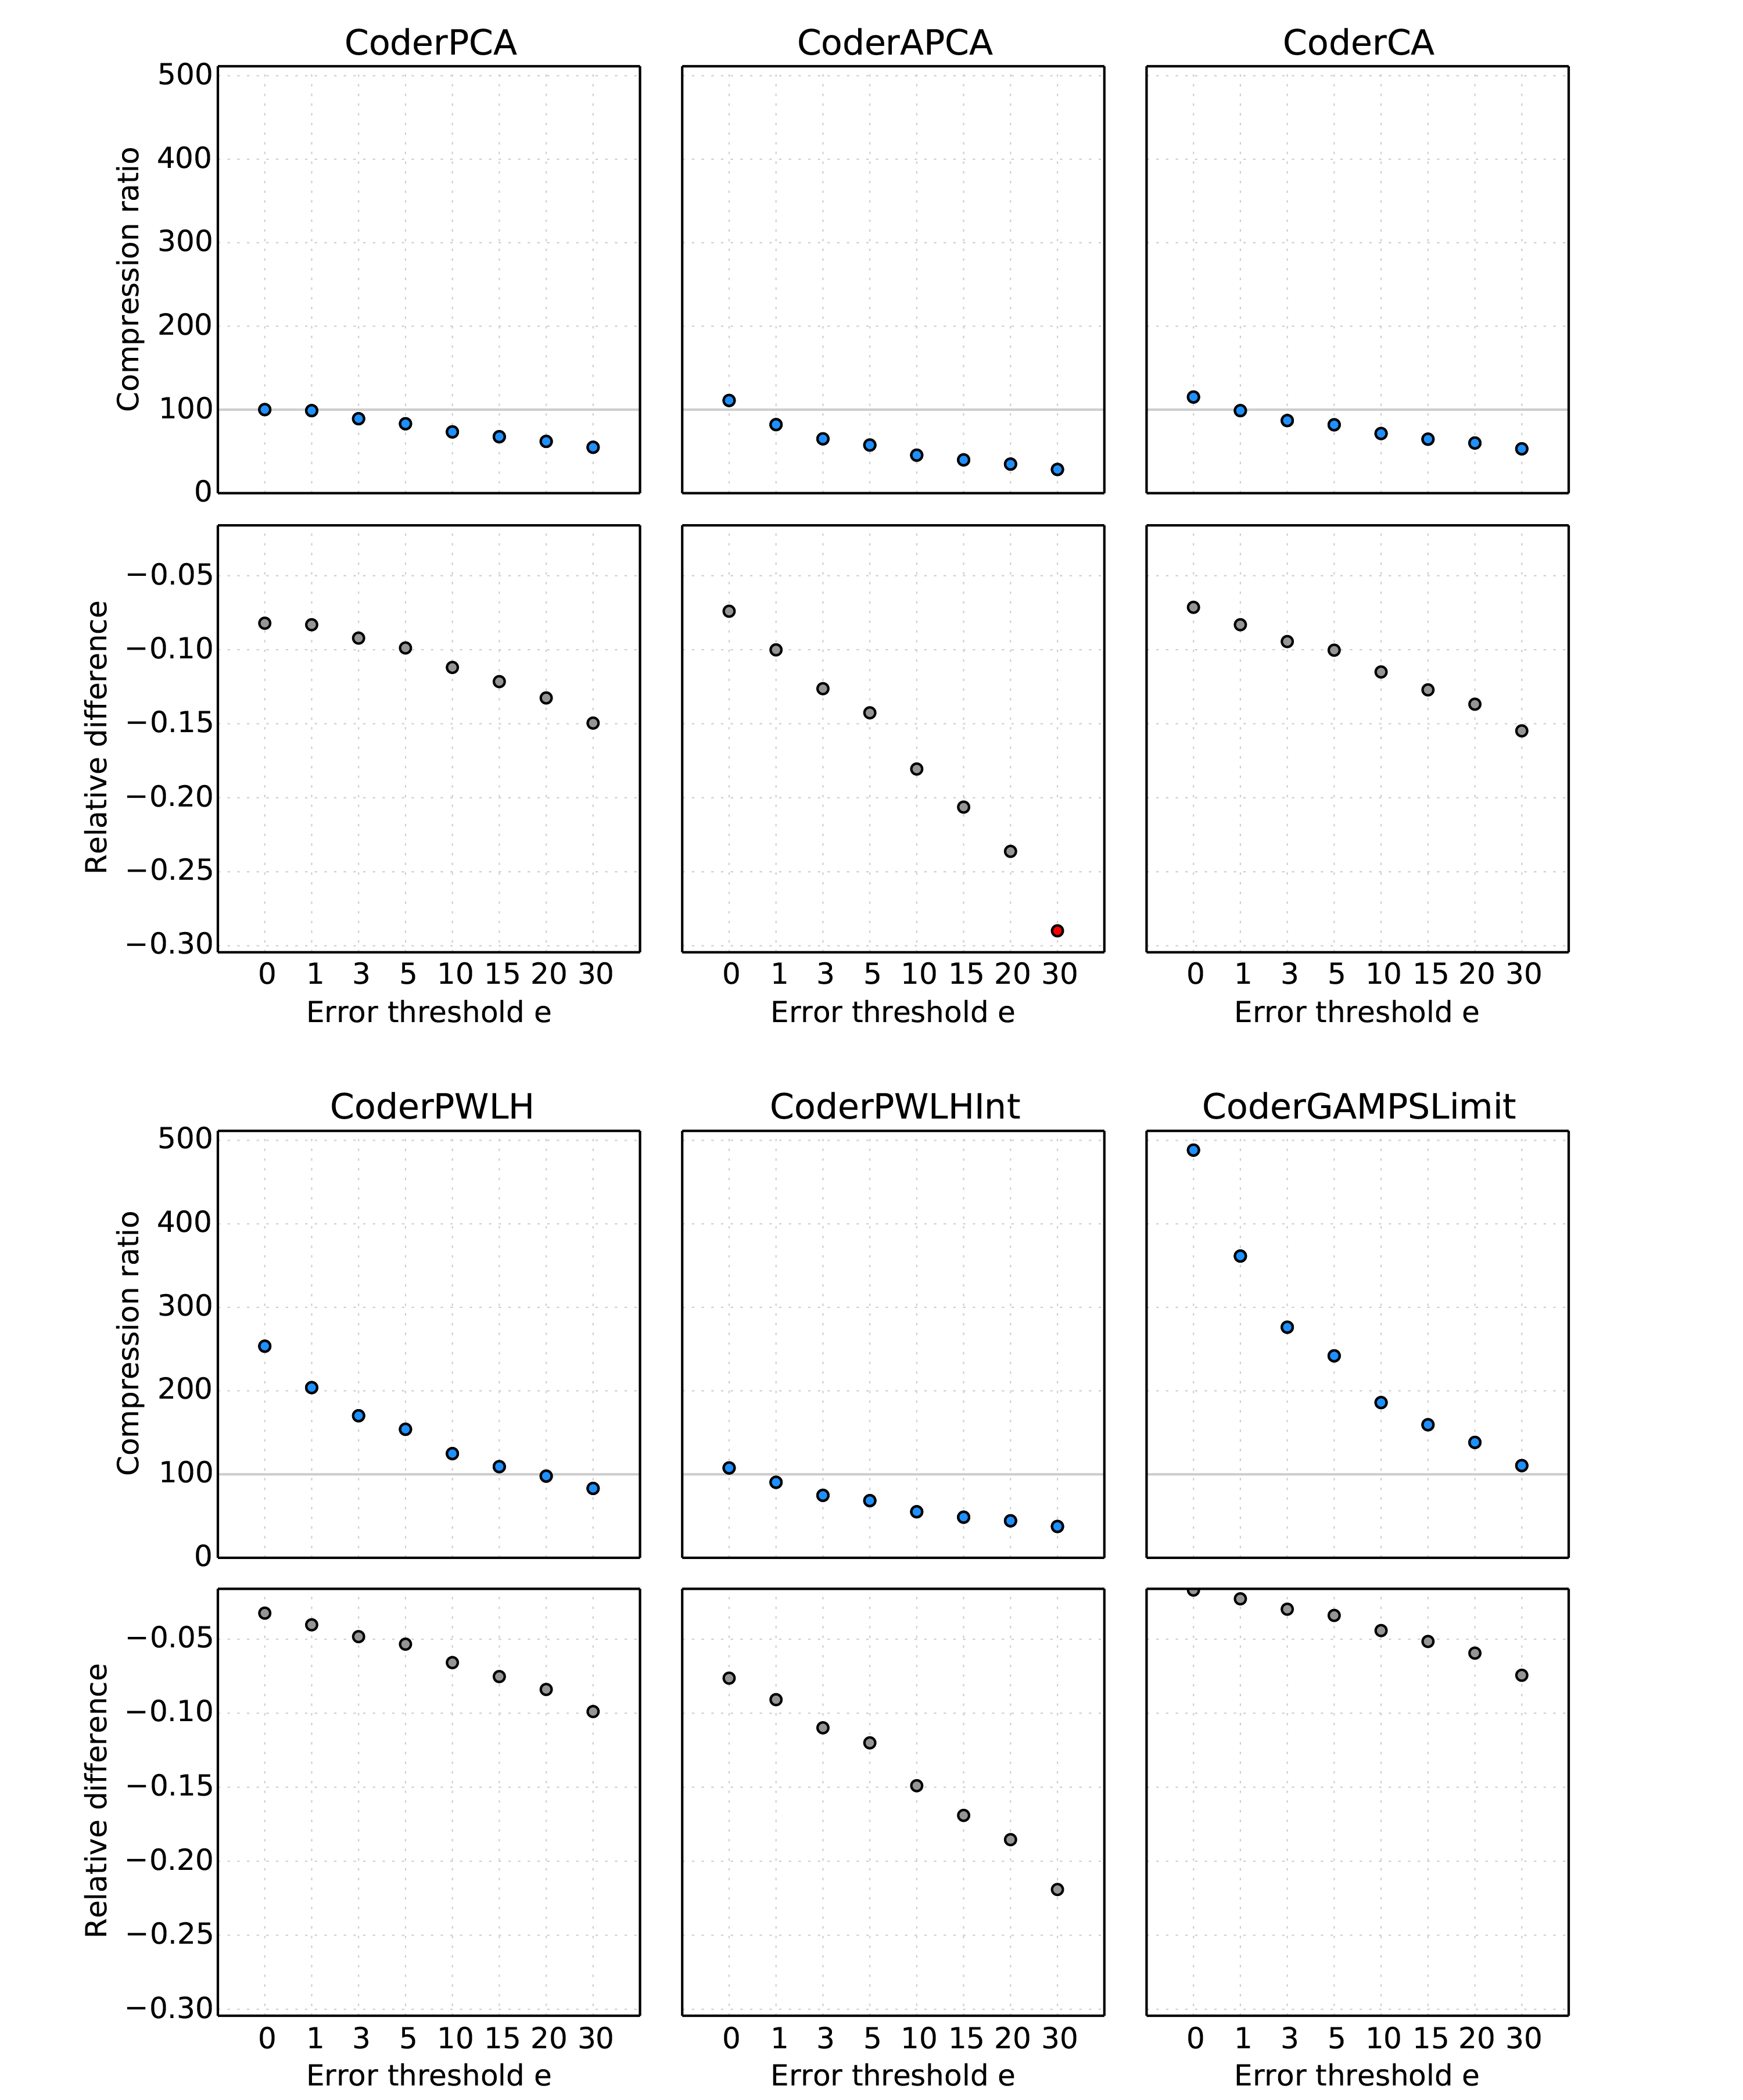
\includegraphics[scale=0.75]{chapters/Experiments/images/32-Tornado.png}
\hspace{+10pt}
\caption{\commonfigurescomp ``Longitude" data type of the \datasettornado \ dataset. In the relative difference plot for\\CoderAPCA we marked with red color the case in which \cNOmaskalgo \ obtains \\the most significant relative difference (-0.29).}
\label{fig:diff-tornado}
\end{figure}

\clearpage

\begin{figure}
\hspace{-70pt}
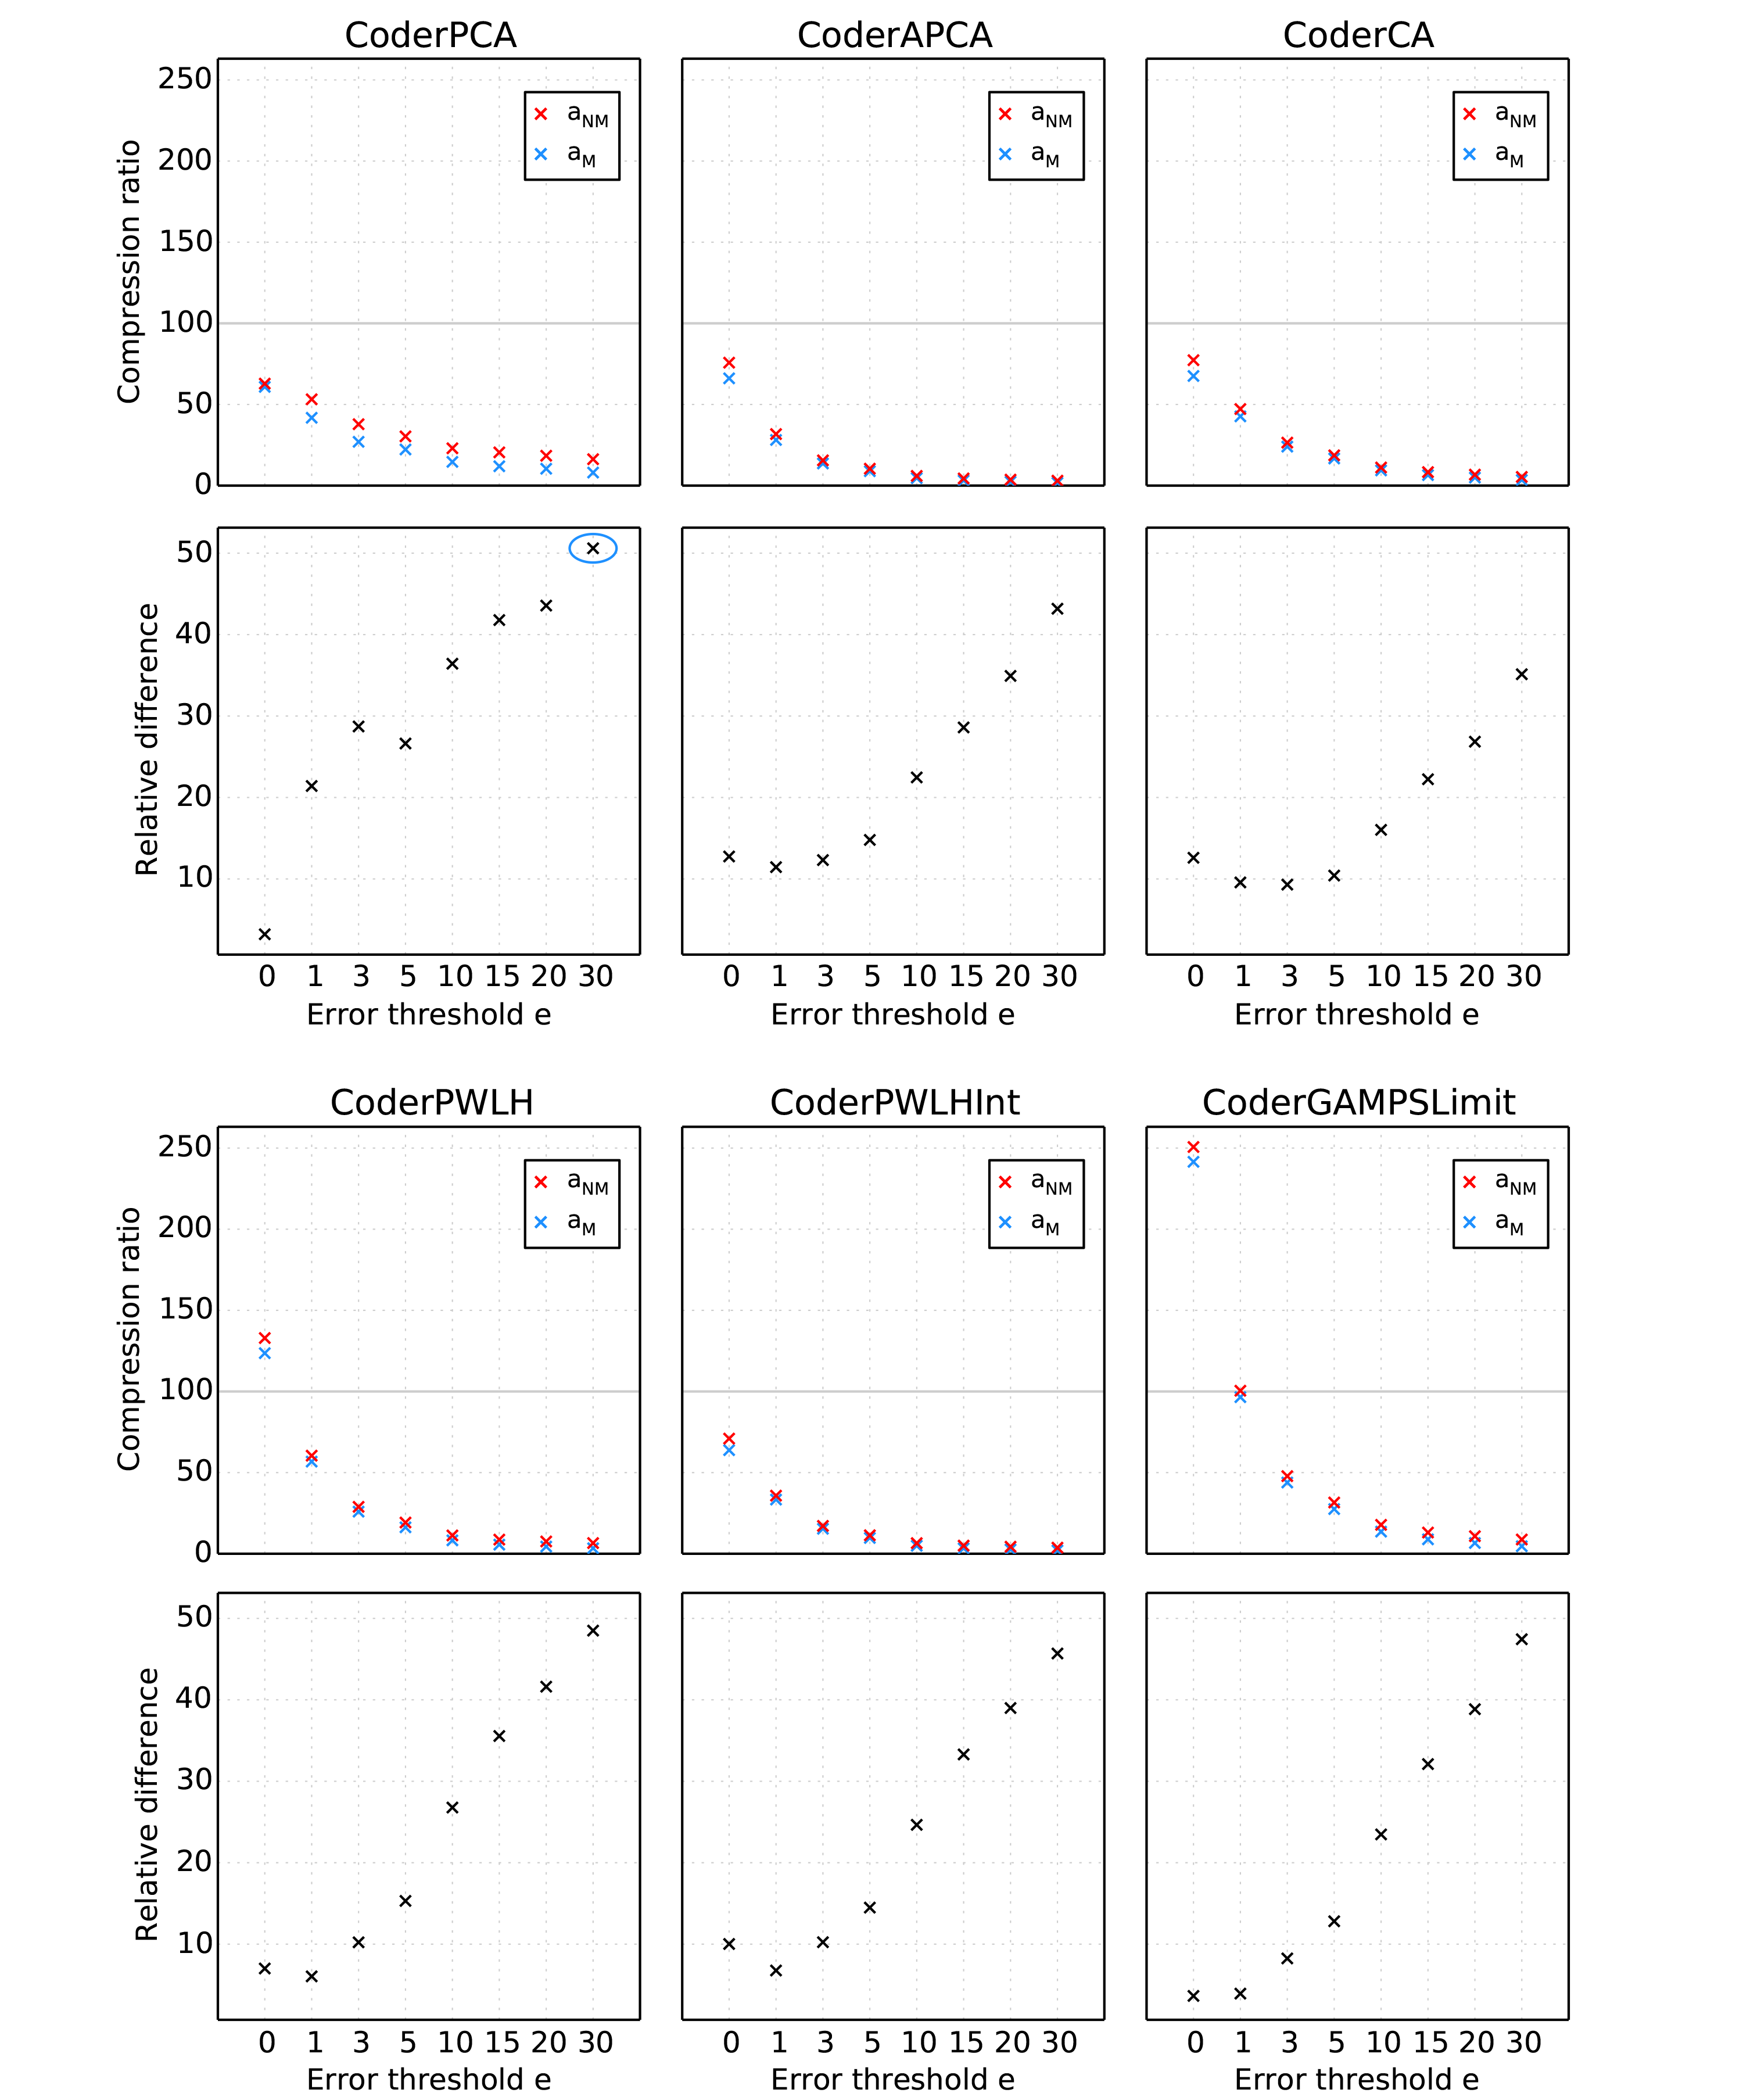
\includegraphics[scale=0.75]{chapters/Experiments/images/32-SST.png}
\hspace{+10pt}
\caption{\commonfigurescomp ``VWC" data type of the \datasetsst \ dataset. In the relative difference plot for\\CoderPCA we marked with blue color the case in which \cmaskalgo \ obtains \\the most significant relative difference (50.60).}
\label{fig:diff-sst}
\end{figure}












\clearpage
\section{Mask Coders Performance}
\label{secX:codersmask}

In this section we analyze the performance of every one of the mask coders implemented in Chapter \ref{coders}. Once again, the compression rate (equation~(\ref{eq:compression-rate})) and the relative difference (equation~(\ref{eq:relative-difference})) will be the metrics we use for comparing the coders between each other.

We considered the results obtained when coding the different data types of the datasets introduced in Chapter \ref{datasets}. For example, in Figure \ref{fig:mask-irkis} we can see the graphs obtained for the ``VWC" data type of the \datasetirkis \ dataset. For each <$\coder \in C$, $e \in E$> combination we plot two values: the window size which minimizes the compression rate and said compression rate.

Easily, after observing the plots we noticed that in general the compression rate for coders \textit{CoderPWLH-M}, \textit{CoderGAMPSLimit-M} and \textit{CoderSF-M} was worst than the rest.

Analyze the data and discard these 

PONER OTRA GRAFICA DE OTRO TIPO DE DATO

\clearpage


\newcommand{\legendsone}{
\begin{tabular}{| C{1.5cm} | C{1.5cm} | C{1.5cm} |}
\hline
  \multicolumn{1}{|>{\centering\arraybackslash}m{1.5cm}|}{\cpca PCA} 
& \multicolumn{1}{>{\centering\arraybackslash}m{1.5cm}|}{\capca APCA} 
& \multicolumn{1}{>{\centering\arraybackslash}m{1.5cm}|}{\cfr FR}\\
\toprule[0.1mm]
\end{tabular}
\vspace{+30pt}
}



\begin{sidewaystable}[ht]
\newcommand{\cgzip}{\cellcolor{orange!20}}
\newcommand{\cfr}{\cellcolor{yellow!25}}
\newcommand{\cpca}{\cellcolor{cyan!20}}
\newcommand{\capca}{\cellcolor{green!20}}
\centering

\legendsone

\begin{tabular}{| l | l | c | c || c | c || c | c || c | c || c | c || c | c || c | c || c | c |}
\cline{3-18}
\multicolumn{1}{c}{}& \multicolumn{1}{c|}{} & \multicolumn{2}{c||}{e = 0} & \multicolumn{2}{c||}{e = 1} & \multicolumn{2}{c||}{e = 3} & \multicolumn{2}{c||}{e = 5} & \multicolumn{2}{c||}{e = 10} & \multicolumn{2}{c||}{e = 15} & \multicolumn{2}{c||}{e = 20} & \multicolumn{2}{c|}{e = 30} \\\hline
{Dataset} & {Data Type} & {\footnotesize OWS} & {\footnotesize CR} & {\footnotesize OWS} & {\footnotesize CR} & {\footnotesize OWS} & {\footnotesize CR} & {\footnotesize OWS} & {\footnotesize CR} & {\footnotesize OWS} & {\footnotesize CR} & {\footnotesize OWS} & {\footnotesize CR} & {\footnotesize OWS} & {\footnotesize CR} & {\footnotesize OWS} & {\footnotesize CR} \\\hline\hline
{\datasetirkis} & {VWC} & {\capca4} & {\capca20.32} & {\capca4} & {\capca18.35} & {\capca5} & {\capca12.37} & {\capca6} & {\capca6.77} & {\capca7} & {\capca3.07} & {\capca8} & {\capca2.22} & {\capca8} & {\capca1.71} & {\capca8} & {\capca1.21} \\\hline
{\datasetsst} & {SST} & {\cpca8} & {\cpca60.84} & {\capca3} & {\capca28.12} & {\capca5} & {\capca13.64} & {\capca6} & {\capca8.88} & {\capca7} & {\capca4.63} & {\capca8} & {\capca3.15} & {\capca8} & {\capca2.39} & {\capca8} & {\capca1.72} \\\hline
{\datasetadcp} & {Vel} & {\cpca8} & {\cpca68.22} & {\cpca8} & {\cpca68.22} & {\capca2} & {\capca66.8} & {\capca2} & {\capca61.07} & {\capca2} & {\capca48.44} & {\capca2} & {\capca40.9} & {\capca3} & {\capca34.9} & {\capca3} & {\capca25.93} \\\hline
{\datasetsolar} & {GHI} & {\cpca2} & {\cpca77.65} & {\capca3} & {\capca76.1} & {\capca4} & {\capca71.39} & {\capca4} & {\capca67.2} & {\capca4} & {\capca58.52} & {\capca4} & {\capca52.41} & {\capca4} & {\capca47.03} & {\capca4} & {\capca37.78} \\\hline
{} & {DNI} & {\cpca2} & {\cpca75.93} & {\capca4} & {\capca72.22} & {\capca4} & {\capca65.75} & {\capca4} & {\capca61.37} & {\capca4} & {\capca53.98} & {\capca4} & {\capca48.55} & {\capca4} & {\capca43.36} & {\capca4} & {\capca35.66} \\\hline
{} & {DHI} & {\cpca2} & {\cpca77.66} & {\cpca2} & {\cpca77.43} & {\capca4} & {\capca71.62} & {\capca4} & {\capca67.6} & {\capca4} & {\capca60.12} & {\capca4} & {\capca53.62} & {\capca4} & {\capca47.86} & {\capca4} & {\capca38.71} \\\hline
{\datasetelnino} & {Lat} & {\capca4} & {\capca15.96} & { } & { } & {\capca4} & {\capca15.82} & {\capca4} & {\capca15.11} & {\capca4} & {\capca12.34} & {\capca5} & {\capca9.89} & {\capca5} & {\capca8.61} & {\capca6} & {\capca5.76} \\\hline
{} & {Long} & {\capca3} & {\capca17.36} & {\capca4} & {\capca17.05} & {\capca4} & {\capca13.04} & {\capca5} & {\capca11.75} & {\capca6} & {\capca8.65} & {\capca6} & {\capca6.56} & {\capca7} & {\capca4.93} & {\capca8} & {\capca2.37} \\\hline
{} & {Zonal Winds} & {\cpca8} & {\cpca31.46} & { } & { } & {\cpca8} & {\cpca31.46} & {\cpca8} & {\cpca31.46} & {\capca2} & {\capca27.36} & {\capca2} & {\capca23.5} & {\capca2} & {\capca20.54} & {\capca3} & {\capca16.44} \\\hline
{} & {Merid. Winds} & {\cpca8} & {\cpca31.46} & { } & { } & {\cpca8} & {\cpca31.46} & {\cpca8} & {\cpca31.46} & {\capca2} & {\capca29.16} & {\capca2} & {\capca25.86} & {\capca2} & {\capca23.33} & {\capca2} & {\capca19.15} \\\hline
{} & {Humidity} & {\cpca8} & {\cpca23.1} & {\cpca8} & {\cpca23.1} & {\cpca8} & {\cpca23.1} & {\cpca8} & {\cpca23.1} & {\capca2} & {\capca20.51} & {\capca2} & {\capca18.14} & {\capca2} & {\capca16.01} & {\capca2} & {\capca12.94} \\\hline
{} & {AirTemp} & {\cpca8} & {\cpca32.68} & {\cpca8} & {\cpca32.68} & {\capca2} & {\capca30.33} & {\capca2} & {\capca27.39} & {\capca2} & {\capca22.42} & {\capca3} & {\capca19.24} & {\capca3} & {\capca16.76} & {\capca4} & {\capca13.31} \\\hline
{} & {SST} & {\cpca8} & {\cpca32.91} & {\capca2} & {\capca30.96} & {\capca2} & {\capca24.6} & {\capca2} & {\capca20.61} & {\capca3} & {\capca14.17} & {\capca4} & {\capca10.66} & {\capca4} & {\capca8.21} & {\capca5} & {\capca5.42} \\\hline
{\datasethail} & {Lat} & {\cpca8} & {\cpca\color{red}100.04} & {\cpca8} & {\cpca\color{red}100.04} & {\capca2} & {\capca89.83} & {\capca2} & {\capca82.62} & {\capca2} & {\capca71.49} & {\capca3} & {\capca64.62} & {\capca3} & {\capca57.49} & {\capca3} & {\capca46.75} \\\hline
{} & {Long} & {\cpca8} & {\cpca\color{red}100.03} & {\cpca8} & {\cpca\color{red}100.03} & {\capca2} & {\capca85.91} & {\capca2} & {\capca77.5} & {\capca2} & {\capca65.06} & {\capca3} & {\capca55.38} & {\capca3} & {\capca48.72} & {\capca4} & {\capca38.74} \\\hline
{} & {Size} & {\capca2} & {\capca80.61} & {\capca2} & {\capca80.59} & {\capca2} & {\capca80.59} & {\capca2} & {\capca80.58} & {\capca2} & {\capca80.56} & {\capca2} & {\capca80.53} & {\capca2} & {\capca80.52} & {\capca3} & {\capca64.35} \\\hline
{\datasettornado} & {Lat} & {\cpca8} & {\cpca\color{red}100.05} & {\capca2} & {\capca85.43} & {\capca2} & {\capca70.63} & {\capca2} & {\capca65.17} & {\capca3} & {\capca54.17} & {\capca3} & {\capca46.78} & {\capca4} & {\capca41.95} & {\capca4} & {\capca33.48} \\\hline
{} & {Long} & {\cpca8} & {\cpca\color{red}100.11} & {\capca2} & {\capca82.12} & {\capca2} & {\capca65.09} & {\capca3} & {\capca57.66} & {\capca3} & {\capca45.55} & {\capca4} & {\capca39.88} & {\capca4} & {\capca34.84} & {\capca4} & {\capca28.41} \\\hline
{\datasetwind} & {Lat} & {\cpca8} & {\cpca\color{red}100.03} & {\cpca8} & {\cpca\color{red}100.03} & {\capca2} & {\capca88.74} & {\capca2} & {\capca81.29} & {\capca2} & {\capca69.82} & {\capca3} & {\capca62.44} & {\capca3} & {\capca56.18} & {\capca3} & {\capca47.15} \\\hline
{} & {Long} & {\cpca8} & {\cpca\color{red}100.03} & {\capca2} & {\capca95.41} & {\capca2} & {\capca80.29} & {\capca2} & {\capca73.21} & {\capca3} & {\capca62.06} & {\capca3} & {\capca54.33} & {\capca3} & {\capca48.52} & {\capca4} & {\capca39.73} \\\hline
{} & {Speed} & {\cfr4} & {\cfr65.49} & {\capca3} & {\capca43.82} & {\cfr6} & {\cfr25.9} & {\cfr7} & {\cfr16.79} & {\capca5} & {\capca15.71} & {\capca6} & {\capca12.29} & {\capca6} & {\capca10.33} & {\capca6} & {\capca8.21} \\\hline
\end{tabular}
\caption{Mask results overview (1).}
\label{experiments:mask-results-overview1}
\end{sidewaystable}



\clearpage
\newcommand{\legendstwo}{
\begin{tabular}{| C{1.5cm} | C{1.5cm} | C{1.5cm} | C{1.5cm} |}
\hline
  \multicolumn{1}{|>{\centering\arraybackslash}m{1.5cm}|}{\cgzip GZIP} 
& \multicolumn{1}{>{\centering\arraybackslash}m{1.5cm}|}{\cpca PCA} 
& \multicolumn{1}{>{\centering\arraybackslash}m{1.5cm}|}{\capca APCA} 
& \multicolumn{1}{>{\centering\arraybackslash}m{1.5cm}|}{\cfr FR}\\
\toprule[0.1mm]
\end{tabular}
\vspace{+30pt}
}

\begin{sidewaystable}[ht]
\newcommand{\cgzip}{\cellcolor{orange!20}}
\newcommand{\cfr}{\cellcolor{yellow!25}}
\newcommand{\cpca}{\cellcolor{cyan!20}}
\newcommand{\capca}{\cellcolor{green!20}}
\centering

\legendstwo


\begin{tabular}{| l | l | c | c || c | c || c | c || c | c || c | c || c | c || c | c || c | c |}
\cline{3-18}
\multicolumn{1}{c}{}& \multicolumn{1}{c|}{} & \multicolumn{2}{c||}{e = 0} & \multicolumn{2}{c||}{e = 1} & \multicolumn{2}{c||}{e = 3} & \multicolumn{2}{c||}{e = 5} & \multicolumn{2}{c||}{e = 10} & \multicolumn{2}{c||}{e = 15} & \multicolumn{2}{c||}{e = 20} & \multicolumn{2}{c|}{e = 30} \\\hline
{Dataset} & {Data Type} & {\footnotesize OWS} & {\footnotesize CR} & {\footnotesize OWS} & {\footnotesize CR} & {\footnotesize OWS} & {\footnotesize CR} & {\footnotesize OWS} & {\footnotesize CR} & {\footnotesize OWS} & {\footnotesize CR} & {\footnotesize OWS} & {\footnotesize CR} & {\footnotesize OWS} & {\footnotesize CR} & {\footnotesize OWS} & {\footnotesize CR} \\\hline\hline
{\datasetirkis} & {VWC} & {\cgzip} & {\cgzip13.44} & {\cgzip} & {\cgzip13.44} & {\capca5} & {\capca12.37} & {\capca6} & {\capca6.77} & {\capca7} & {\capca3.07} & {\capca8} & {\capca2.22} & {\capca8} & {\capca1.71} & {\capca8} & {\capca1.21} \\\hline
{\datasetsst} & {SST} & {\cgzip} & {\cgzip52.06} & {\capca3} & {\capca28.12} & {\capca5} & {\capca13.64} & {\capca6} & {\capca8.88} & {\capca7} & {\capca4.63} & {\capca8} & {\capca3.15} & {\capca8} & {\capca2.39} & {\capca8} & {\capca1.72} \\\hline
{\datasetadcp} & {Vel} & {\cgzip} & {\cgzip61.38} & {\cgzip} & {\cgzip61.38} & {\cgzip} & {\cgzip61.38} & {\capca2} & {\capca61.07} & {\capca2} & {\capca48.44} & {\capca2} & {\capca40.9} & {\capca3} & {\capca34.9} & {\capca3} & {\capca25.93} \\\hline
{\datasetsolar} & {GHI} & {\cgzip} & {\cgzip69.01} & {\cgzip} & {\cgzip69.01} & {\cgzip} & {\cgzip69.01} & {\capca4} & {\capca67.2} & {\capca4} & {\capca58.52} & {\capca4} & {\capca52.41} & {\capca4} & {\capca47.03} & {\capca4} & {\capca37.78} \\\hline
{} & {DNI} & {\cgzip} & {\cgzip66.88} & {\cgzip} & {\cgzip66.88} & {\capca4} & {\capca65.75} & {\capca4} & {\capca61.37} & {\capca4} & {\capca53.98} & {\capca4} & {\capca48.55} & {\capca4} & {\capca43.36} & {\capca4} & {\capca35.66} \\\hline
{} & {DHI} & {\cgzip} & {\cgzip61.01} & {\cgzip} & {\cgzip61.01} & {\cgzip} & {\cgzip61.01} & {\cgzip} & {\cgzip61.01} & {\capca4} & {\capca60.12} & {\capca4} & {\capca53.62} & {\capca4} & {\capca47.86} & {\capca4} & {\capca38.71} \\\hline
{\datasetelnino} & {Lat} & {\cgzip} & {\cgzip7.89} & { } & { } & {\cgzip} & {\cgzip7.89} & {\cgzip} & {\cgzip7.89} & {\cgzip} & {\cgzip7.89} & {\cgzip} & {\cgzip7.89} & {\cgzip} & {\cgzip7.89} & {\capca6} & {\capca5.76} \\\hline
{} & {Long} & {\cgzip} & {\cgzip7.1} & {\cgzip} & {\cgzip7.1} & {\cgzip} & {\cgzip7.1} & {\cgzip} & {\cgzip7.1} & {\cgzip} & {\cgzip7.1} & {\capca6} & {\capca6.56} & {\capca7} & {\capca4.93} & {\capca8} & {\capca2.37} \\\hline
{} & {Zonal Winds} & {\cpca8} & {\cpca31.46} & { } & { } & {\cpca8} & {\cpca31.46} & {\cpca8} & {\cpca31.46} & {\capca2} & {\capca27.36} & {\capca2} & {\capca23.5} & {\capca2} & {\capca20.54} & {\capca3} & {\capca16.44} \\\hline
{} & {Merid. Winds} & {\cpca8} & {\cpca31.46} & { } & { } & {\cpca8} & {\cpca31.46} & {\cpca8} & {\cpca31.46} & {\capca2} & {\capca29.16} & {\capca2} & {\capca25.86} & {\capca2} & {\capca23.33} & {\capca2} & {\capca19.15} \\\hline
{} & {Humidity} & {\cpca8} & {\cpca23.1} & {\cpca8} & {\cpca23.1} & {\cpca8} & {\cpca23.1} & {\cpca8} & {\cpca23.1} & {\capca2} & {\capca20.51} & {\capca2} & {\capca18.14} & {\capca2} & {\capca16.01} & {\capca2} & {\capca12.94} \\\hline
{} & {AirTemp} & {\cpca8} & {\cpca32.68} & {\cpca8} & {\cpca32.68} & {\capca2} & {\capca30.33} & {\capca2} & {\capca27.39} & {\capca2} & {\capca22.42} & {\capca3} & {\capca19.24} & {\capca3} & {\capca16.76} & {\capca4} & {\capca13.31} \\\hline
{} & {SST} & {\cgzip} & {\cgzip32.43} & {\capca2} & {\capca30.96} & {\capca2} & {\capca24.6} & {\capca2} & {\capca20.61} & {\capca3} & {\capca14.17} & {\capca4} & {\capca10.66} & {\capca4} & {\capca8.21} & {\capca5} & {\capca5.42} \\\hline
{\datasethail} & {Lat} & {\cpca8} & {\cpca\color{red}100.04} & {\cpca8} & {\cpca\color{red}100.04} & {\capca2} & {\capca89.83} & {\capca2} & {\capca82.62} & {\capca2} & {\capca71.49} & {\capca3} & {\capca64.62} & {\capca3} & {\capca57.49} & {\capca3} & {\capca46.75} \\\hline
{} & {Long} & {\cpca8} & {\cpca\color{red}100.03} & {\cpca8} & {\cpca\color{red}100.03} & {\capca2} & {\capca85.91} & {\capca2} & {\capca77.5} & {\capca2} & {\capca65.06} & {\capca3} & {\capca55.38} & {\capca3} & {\capca48.72} & {\capca4} & {\capca38.74} \\\hline
{} & {Size} & {\cgzip} & {\cgzip36.73} & {\cgzip} & {\cgzip36.73} & {\cgzip} & {\cgzip36.73} & {\cgzip} & {\cgzip36.73} & {\cgzip} & {\cgzip36.73} & {\cgzip} & {\cgzip36.73} & {\cgzip} & {\cgzip36.73} & {\cgzip} & {\cgzip36.73} \\\hline
{\datasettornado} & {Lat} & {\cpca8} & {\cpca\color{red}100.05} & {\capca2} & {\capca85.43} & {\capca2} & {\capca70.63} & {\capca2} & {\capca65.17} & {\capca3} & {\capca54.17} & {\capca3} & {\capca46.78} & {\capca4} & {\capca41.95} & {\capca4} & {\capca33.48} \\\hline
{} & {Long} & {\cpca8} & {\cpca\color{red}100.11} & {\capca2} & {\capca82.12} & {\capca2} & {\capca65.09} & {\capca3} & {\capca57.66} & {\capca3} & {\capca45.55} & {\capca4} & {\capca39.88} & {\capca4} & {\capca34.84} & {\capca4} & {\capca28.41} \\\hline
{\datasetwind} & {Lat} & {\cpca8} & {\cpca\color{red}100.03} & {\cpca8} & {\cpca\color{red}100.03} & {\capca2} & {\capca88.74} & {\capca2} & {\capca81.29} & {\capca2} & {\capca69.82} & {\capca3} & {\capca62.44} & {\capca3} & {\capca56.18} & {\capca3} & {\capca47.15} \\\hline
{} & {Long} & {\cpca8} & {\cpca\color{red}100.03} & {\capca2} & {\capca95.41} & {\capca2} & {\capca80.29} & {\capca2} & {\capca73.21} & {\capca3} & {\capca62.06} & {\capca3} & {\capca54.33} & {\capca3} & {\capca48.52} & {\capca4} & {\capca39.73} \\\hline
{} & {Speed} & {\cfr4} & {\cfr65.49} & {\capca3} & {\capca43.82} & {\cfr6} & {\cfr25.9} & {\cfr7} & {\cfr16.79} & {\capca5} & {\capca15.71} & {\capca6} & {\capca12.29} & {\capca6} & {\capca10.33} & {\capca6} & {\capca8.21} \\\hline
\end{tabular}
\caption{Mask results overview (2).}
\label{experiments:mask-results-overview2}
\end{sidewaystable}




\clearpage
\begin{figure}
\hspace{-35pt}
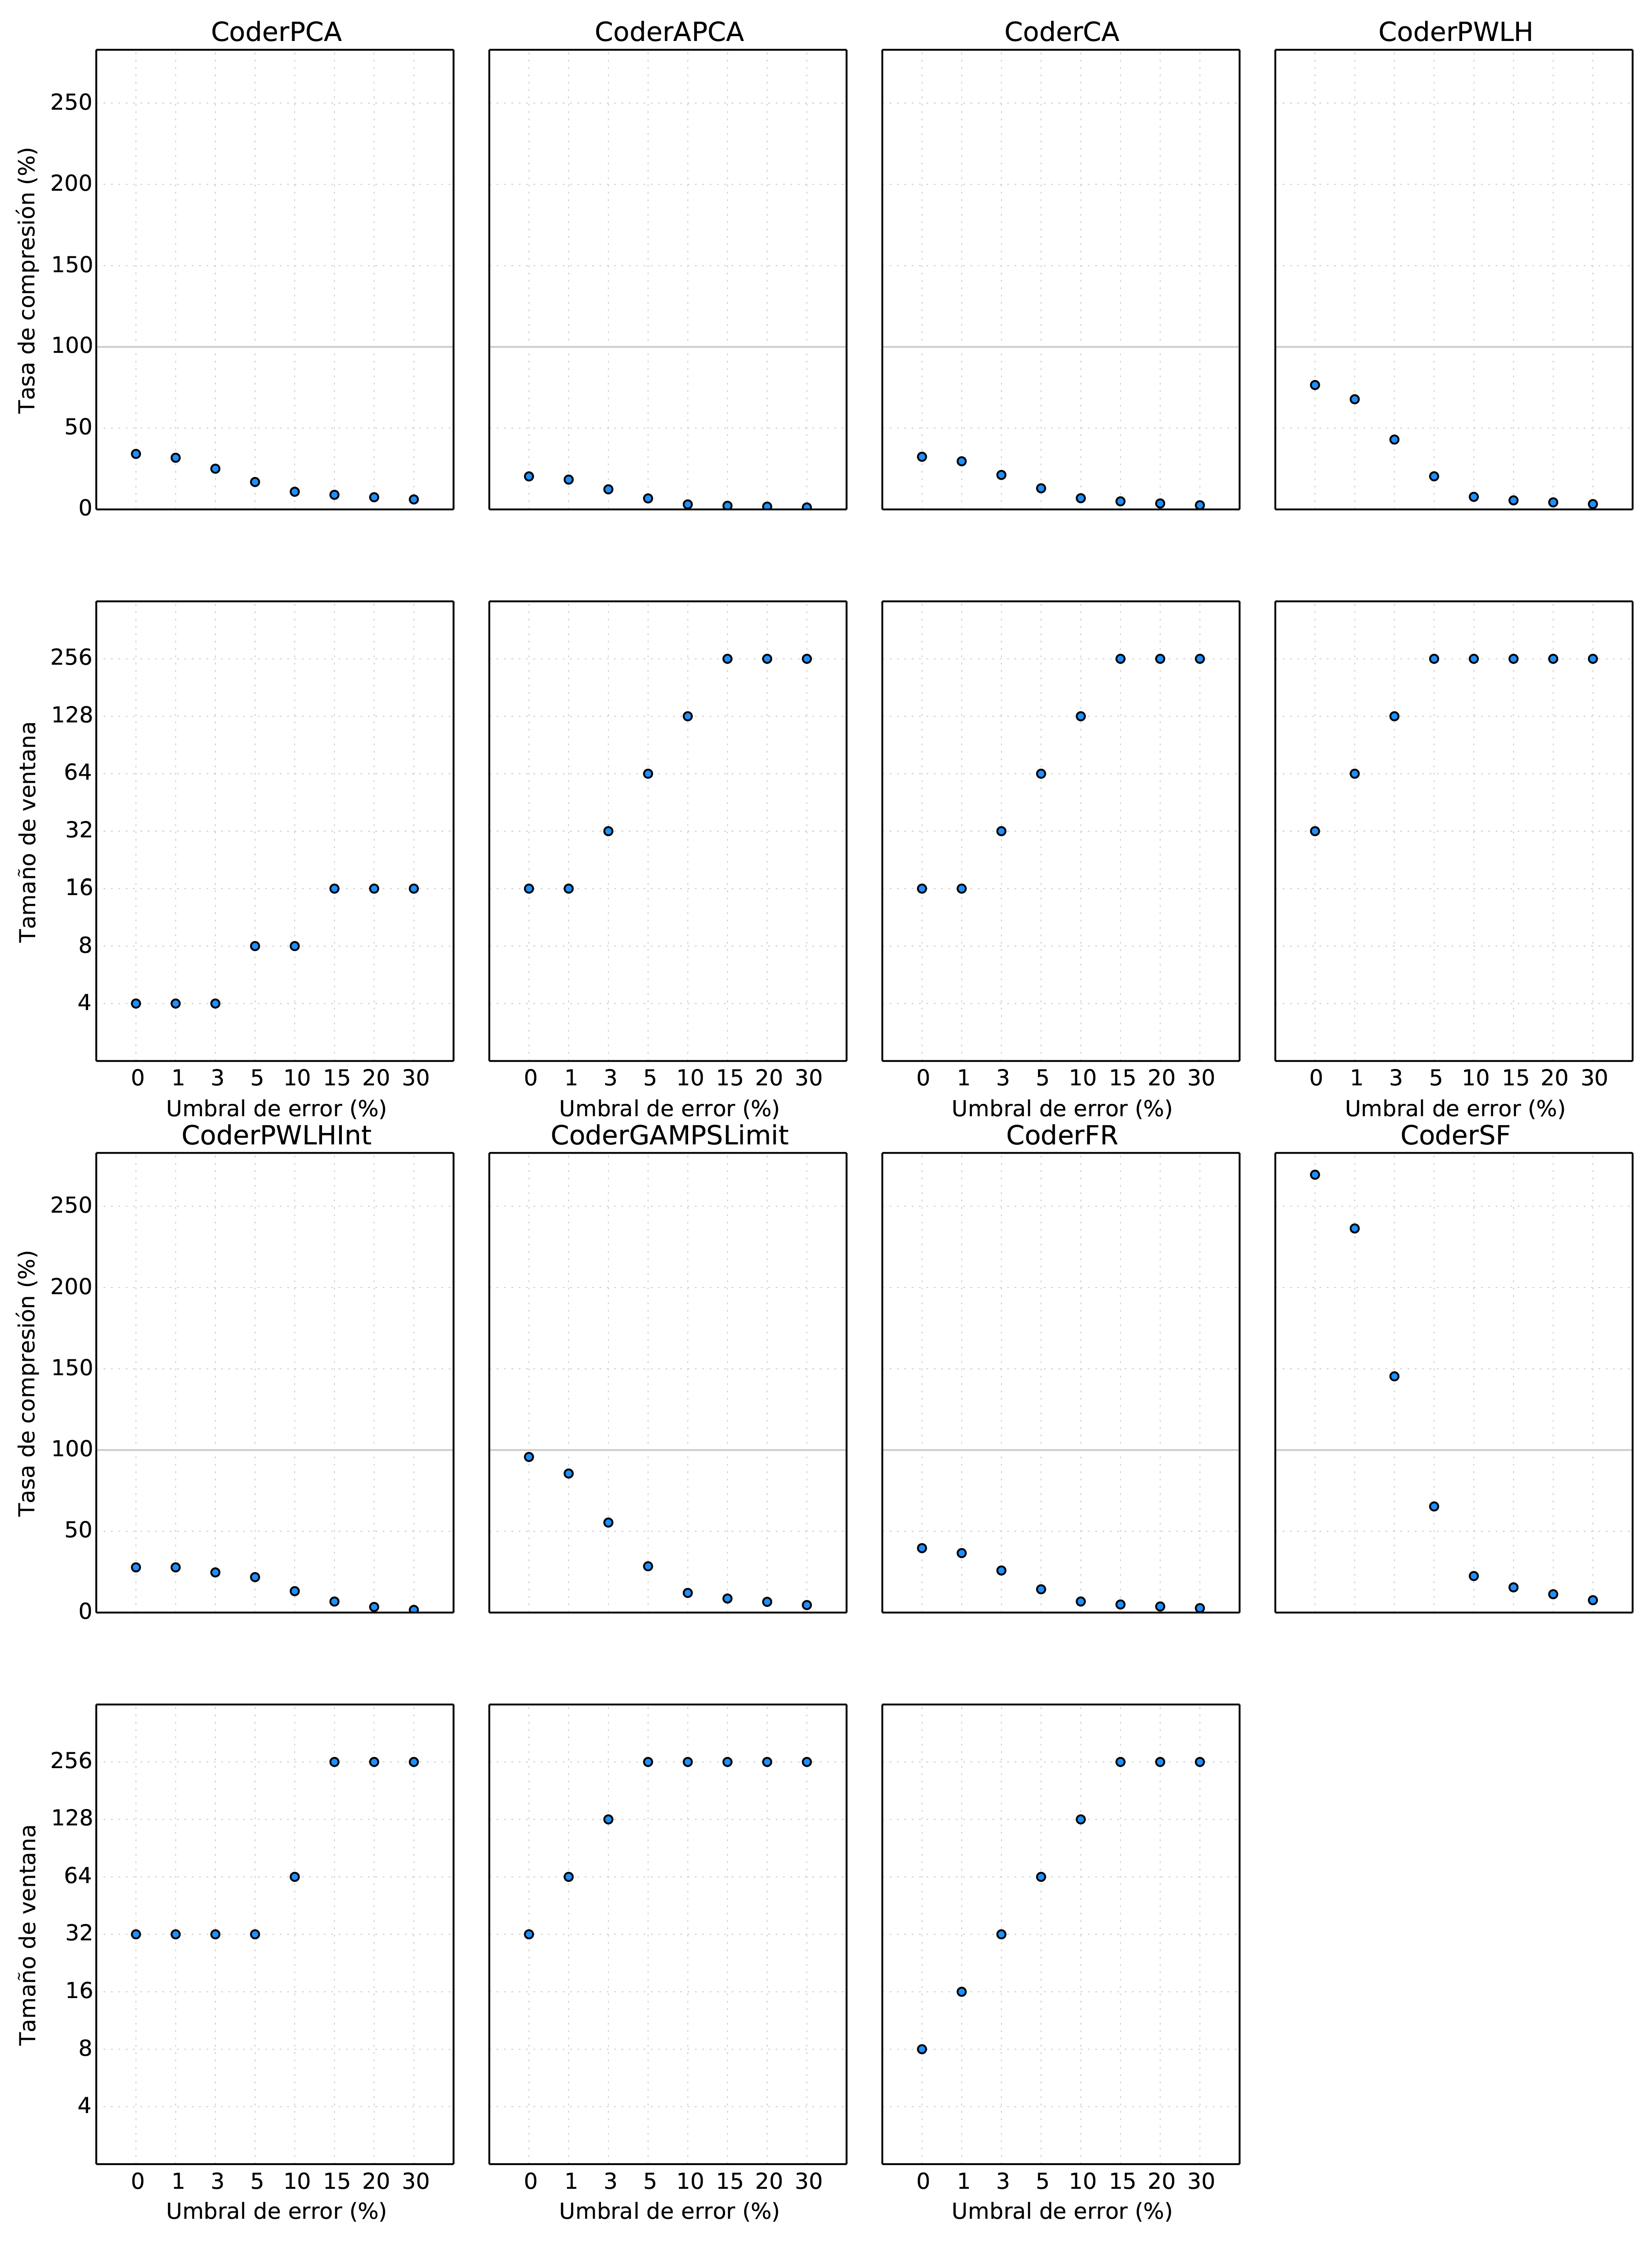
\includegraphics[scale=0.50]{chapters/Experiments/images/1-IRKIS.png}
\hspace{+10pt}
\caption{Compression rate and Window size graphs for the different combinations\\<$\coder \in C$, $w \in W, e \in E$> for the ``VWC" data type of the \datasetirkis \ dataset.}
\label{fig:mask-irkis}
\end{figure}

\clearpage







\clearpage
\section{Comparison with the gzip Algorithm}
\label{secX:gzip}